%----------------------------------------------------------------------------------------
%	DOCUMENT CONFIGURATIONS
%----------------------------------------------------------------------------------------

\documentclass[a4paper,12pt]{report}
\usepackage[francais]{babel}
\usepackage[utf8]{inputenc}
\usepackage[T1]{fontenc}
\usepackage{ucs}
\usepackage{url}
\usepackage{graphicx}
\usepackage[table]{xcolor}
\usepackage{mathtools,amssymb,amsthm}%
\usepackage[left=2.5cm,top=2cm,right=2.5cm,nohead,nofoot]{geometry}
\usepackage{pdfpages}
\usepackage[table]{xcolor}
\usepackage{color}
\usepackage{algorithm}
\usepackage{algpseudocode}
\usepackage{array}
\usepackage{graphicx}
\usepackage{caption}
\usepackage{subcaption}
\linespread{1.1}
%%%%%%%%%%%%%%%%%
\makeatletter
\newif\if@borderstar
\def\bordermatrix{\@ifnextchar*{%
\@borderstartrue\@bordermatrix@i}{\@borderstarfalse\@bordermatrix@i*}%
}
\def\@bordermatrix@i*{\@ifnextchar[{\@bordermatrix@ii}{\@bordermatrix@ii[()]}}
\def\@bordermatrix@ii[#1]#2{%
\begingroup
\m@th\@tempdima8.75\p@\setbox\z@\vbox{%
\def\cr{\crcr\noalign{\kern 2\p@\global\let\cr\endline }}%
\ialign {$##$\hfil\kern 2\p@\kern\@tempdima & \thinspace %
\hfil $##$\hfil && \quad\hfil $##$\hfil\crcr\omit\strut %
\hfil\crcr\noalign{\kern -\baselineskip}#2\crcr\omit %
\strut\cr}}%
\setbox\tw@\vbox{\unvcopy\z@\global\setbox\@ne\lastbox}%
\setbox\tw@\hbox{\unhbox\@ne\unskip\global\setbox\@ne\lastbox}%
\setbox\tw@\hbox{%
$\kern\wd\@ne\kern -\@tempdima\left\@firstoftwo#1%
\if@borderstar\kern2pt\else\kern -\wd\@ne\fi%
\global\setbox\@ne\vbox{\box\@ne\if@borderstar\else\kern 2\p@\fi}%
\vcenter{\if@borderstar\else\kern -\ht\@ne\fi%
\unvbox\z@\kern-\if@borderstar2\fi\baselineskip}%
\if@borderstar\kern-2\@tempdima\kern2\p@\else\,\fi\right\@secondoftwo#1 $%
}\null \;\vbox{\kern\ht\@ne\box\tw@}%
\endgroup
}
\makeatother
%%%%%%%%%%%%%%%%%
\newcommand\black{\cellcolor{black}}
\newcommand\grey{\cellcolor{black!50}}

%%%%%%%%%%%%%%%%%

\usepackage{listings}
\definecolor{lightgray}{rgb}{.9,.9,.9}
\definecolor{darkgray}{rgb}{.4,.4,.4}
\definecolor{purple}{rgb}{0.65, 0.12, 0.82}
\lstdefinestyle{Cpp}{
backgroundcolor=\color{lightgray},
  belowcaptionskip=1\baselineskip,
  breaklines=true,
  captionpos=b,
  xleftmargin=\parindent,
  language=C++,
  numbers=left,
  numbersep=5pt,
  numberstyle=\tiny\color{darkgray},
  showstringspaces=false,
  basicstyle=\footnotesize\ttfamily,
  keywordstyle=\bfseries\color{green!40!black},
  commentstyle=\itshape\color{purple!40!black},
  identifierstyle=\color{blue},
  stringstyle=\color{orange},
}
%%%%%%%%%%%%%%%%%%%%%%%%%%%%%%%%%%%%%%%%%%%%%

% verbatim boxed text
\usepackage{fancyvrb,fancybox,calc} 
%\usepackage[svgnames]{xcolor} 
\newenvironment{bash}{\VerbatimEnvironment% 

  \noindent
  %      {\columnwidth-\leftmargin-\rightmargin-2\fboxsep-2\fboxrule-4pt} 
  \begin{Sbox} 
  \begin{minipage}[c]{\textwidth}%\linewidth-2\fboxsep-2\fboxrule-4pt}    
  \begin{Verbatim}
}{% 
  \end{Verbatim}  
  \end{minipage}   
  \end{Sbox} 
  \fcolorbox{gray}{LightGray}{\TheSbox} 
} 
%%%%%%%%%%%%%%%%%%%%%%%%%%%%%%%%%%%%%%%%%%%%%\color{declared-color}
% verbatim boxed text
\newenvironment{command}{\VerbatimEnvironment% 

  \noindent
  %      {\columnwidth-\leftmargin-\rightmargin-2\fboxsep-2\fboxrule-4pt} 
  \begin{Sbox} 
  \begin{minipage}[c]{\textwidth}%\linewidth-2\fboxsep-2\fboxrule-4pt} 
  \color{white}   
  \begin{Verbatim}
}{% 
  \end{Verbatim}  
  \end{minipage}   
  \end{Sbox} 
  \fcolorbox{black}{gray}{\TheSbox} 
} 
%%%%%%%%%%%%%%%%%%%%%%%%%%%%%%%%%%%%%%%%%%%%%

\begin{document}


\setlength\parindent{0pt} % Removes all indentation from paragraphs


\begin{titlepage}
\begin{center}
\textbf{\textsc{UNIVERSIT\'E LIBRE DE BRUXELLES}}\\
\textbf{\textsc{Faculté des Sciences}}\\
\textbf{\textsc{Département d'Informatique}}
\vfill{}\vfill{}
\begin{center}{\Huge INFO-F-302 - Logique Informatique \\Projet: Le jeu Pattern\\ et\\ Utilisation de MiniSAT}\end{center}{\Huge \par}
\begin{center}{\large \textsc{Ooms} Aurélien, \textsc{Sonnet} Jean-Baptiste}\end{center}{\Huge \par}
\vfill{}\vfill{}
\vfill{}\vfill{}\enlargethispage{3cm}
\textbf{Année académique 2012~-~2013}
\end{center}
\end{titlepage}




\tableofcontents
\newpage


\chapter{Question 1: Énumération 3,2}

\section{Problème et notation}
\subsection{Grille}
Le problème est présenté sous forme d'une grille $3\times3$ contenant au $max$ 2 contraintes par ligne ou colonne.\\

Soit une matrice $3\times3$,  
$$\begin{bmatrix} x_{0,0} & x_{0,1} & x_{0,2} \\ x_{1,0} & x_{1,1} & x_{1,2} \\ x_{2,0} & x_{2,1} & x_{2,2}\end{bmatrix} \rightarrow \begin{bmatrix} 1 & 2 & 3 \\ 4 & 5 & 6 \\ 7 & 8 & 9\end{bmatrix}$$ 
où chacune des cases $x_{i,j}$ prendra potentiellement une des 2 valeurs: 
$\{-1,1\}$, respectivement le blanc, le noir. Les cases sont initialisées avec la valeur $0$.\\

On aura par exemple comme problème à résoudre:
\begin{center}
$\bordermatrix[{[]}]{
	\text{ }	 
		& 2		& 1		& 2		\cr
1	 	& 1		& -1 	& 0		\cr
1\; 1  	& 0 	& 0 	& 0		\cr
2    	& 0 	& 0 	& 0		\cr
} $
\begin{tabular}{|c|c|c|}
\hline 
\black• &   & \grey?  \\ 
\hline 
\grey? & \grey?  & \grey? \\ 
\hline 
\grey? & \grey? & \grey? \\ 
\hline 
\end{tabular}
\end{center}

Selon les contraintes précisées, la solution devra donner pour toutes les cases inconnues une valeur de $1$ ou $-1$:\\
\begin{center}
$\bordermatrix[{[]}]{
	\text{ }	 
		& 2		& 1		& 2		\cr
1	 	& 1		& -1 	& -1	\cr
1\; 1  	& 1 	& -1 	& 1		\cr
2    	& -1 	& 1 	& 1		\cr
}$
\begin{tabular}{|c|c|c|}
\hline 
\black• &  &  \\ 
\hline 
\black• &  & \black• \\ 
\hline 
 & \black• & \black• \\ 
\hline 
\end{tabular}
\end{center}
\subsection{Variables}
Chaque case est représentée par une variable $x$, de sorte que la case à la $i^{eme}$ ligne et à la $j^{eme}$ colonne se note $x_{i,j}$.\\

On a que $(i,j)\in \{1,2,3\}^2$ et que chaque variable peut prendre comme valeur $v \in \{-1,0,1\}$
soit:
$$X=\{x_{i,j}| (i,j)\in \{0,1,2\}^2, v \in \{-1,0,1\}\}$$
\subsection{Sémantique}
On a pour sémantique: 
\begin{itemize}
\item $x_{i,j}$ est \textbf{vrai} \textit{si et seulement si} la case $(i,j)$ a pour valeur $v=1$
\item $x_{i,j}$ est \textbf{faux} \textit{si et seulement si} la case $(i,j)$ a pour valeur $v=-1$
\end{itemize}

\subsection{Codage}
Pour miniSAT, il faut coder les propositions par des entiers.


La taille d'une grille est $3\times3$, pour $x_{i,j}$ on aurait par exemple le codage: $(i \times 3)+ j$


\section{Contraintes}
\begin{enumerate}

\item (trivial) \textbf{Pour chaque} ligne, s'il existe une bande, \textbf{toutes} les cases ne sont pas fausses.
$$ \bigwedge_{i \in \{0,1,2\}} \lnot \left( \bigwedge_{j \in \{0,1,2\}} \lnot x_{i,j} \right) $$
soit,
$$ \bigwedge_{i \in \{0,1,2\}} \left( \bigvee_{j \in \{0,1,2\}} x_{i,j} \right) $$
idem pour chaque colonne.
$$ \bigwedge_{j \in \{0,1,2\}} \left( \bigvee_{i \in \{0,1,2\}} x_{i,j} \right) $$

\item (trivial) \textbf{Pour toute} ligne, \textbf{pour toute} colonne, \textbf{pour toute} bande, \textbf{il existe} une case qui satisfait à la fois une bande de la ligne et une de la colonne.
$$\bigwedge_{i \in \{0,1,2\}} \bigwedge_{j \in \{0,1,2\}} \bigwedge_{b_i^{(k)}, k\in\{1,2\}} 
\lnot \left(
	\lnot x_{i,j} \wedge x_{i,j}
\right)$$
soit,
$$\bigwedge_{i \in \{0,1,2\}} \bigwedge_{j \in \{0,1,2\}} \bigwedge_{b_i^{(k)}, k\in\{1,2\}} 
\left(
	x_{i,j} \vee \lnot x_{i,j}
\right)$$

\item \textbf{Pour toute} ligne $i$, \textbf{pour toute} bande de taille $b$ associée à la ligne, \textbf{il existe} \textit{autant} de cases vraies $x_{i,j}$ que ne l'exprime la taille de chaque bande. 

Cela donne au cas par cas:
	\begin{enumerate}
		\item Une seule bande: 
		\begin{enumerate}
			\item Pour toute ligne $i$ où $b=3$, 
			$$\bigwedge_{j\in\{0,1,2\}}\left( \bigvee_{l=1}^{n=1} x_{i,j} \right)$$
			\begin{center}						
			\begin{tabular}{|c|c|c|}
			\hline 
			$\top$ & $\top$  & $\top$  \\ 
			\hline  
			\end{tabular}
			\end{center}

			\item Pour toute ligne $i$ où $b=2$, 
			$$(\lnot x_{i,0} \vee \lnot x_{i,2}) \wedge x_{i,1}\wedge (x_{i,0} \vee x_{i,2}) $$
			\begin{center}						
			\begin{tabular}{|c|c|c|}
			\hline 
			$\top$ & $\top$  & $\bot$  \\ 
			\hline  
			\end{tabular}
			ou
			\begin{tabular}{|c|c|c|}
			\hline 
			$\bot$ & $\top$  & $\top$  \\ 
			\hline  
			\end{tabular}
			\end{center}
			
			\item Pour toute ligne $i$ où $b=1$, 
			$$\bigwedge_{\stackrel{j,j' \in\{0,1,2\}}{j<j', j''\neq j,j'}} (\lnot x_{i,j}\vee \lnot x_{i,j'} \vee x_{i,j''} ) $$
			\begin{center}						
			\begin{tabular}{|c|c|c|}
			\hline 
			$\top$ & $\bot$  & $\bot$  \\ 
			\hline  
			\end{tabular}
			ou
			\begin{tabular}{|c|c|c|}
			\hline 
			$\bot$ & $\top$  & $\bot$  \\ 
			\hline  
			\end{tabular}
			ou
			\begin{tabular}{|c|c|c|}
			\hline 
			$\bot$ & $\bot$  & $\top$  \\ 
			\hline  
			\end{tabular}
			\end{center}
			
			\item Pour toute ligne $i$ où $b=0$,
			$$\bigwedge_{j\in\{0,1,2\}}\left( \bigvee_{l=1}^{n=1} \lnot x_{i,j} \right)$$
			où $\bigvee_{l=1}^{n=1}$ précise qu'on a une FNC.
			\begin{center}						
			\begin{tabular}{|c|c|c|}
			\hline 
			$\bot$ & $\bot$  & $\bot$  \\ 
			\hline  
			\end{tabular}
			\end{center}
			
		\end{enumerate}

		\item Deux bandes, pour toute ligne $i$:
		$$\left( \bigvee_{l=1}^{n=1} x_{i,0} \right) \wedge \left(\bigvee_{l=1}^{n=1} \lnot x_{i,1}\right) \wedge \left(\bigvee_{l=1}^{n=1} x_{i,2}\right)$$
			\begin{center}						
			\begin{tabular}{|c|c|c|}
			\hline 
			$\top$ & $\bot$  & $\top$  \\ 
			\hline  
			\end{tabular}
			\end{center}
			
	\end{enumerate}
	Idem pour toute colonne. 
\end{enumerate}

\section{Parcours et représentation par énumération}


On va parcourir la grille et énumérer les combinaisons possibles premièrement suivant les contraintes de lignes ensuite selon les contraintes de colonnes.\\ 

Par ligne (respectivement colonne), on crée si nécessaire une clause représentant les cas possibles quant aux cases dont on ne connait pas encore la nature.\\

Pour chaque case contenue dans une ligne $i$ donnée:
\begin{enumerate}
\item Si elle contient une information ($1$ ou $-1$), on en créer une clause à part entière qui sera jointe ($\wedge$) à toutes les autres.
\item Si elle ne contient pas d'informations ($0$) et conditionnellement au contraintes $c_i^{(k)}, k\in\{1,2\}$, on énumère les possibilités sous forme disjonctive.\\
\end{enumerate}
On effectue de même par colonne et relativement aux contraintes de la colonne.\\


%L'énumération des cas possibles se formule naturellement à l'aide de la disjonction exclusive (XOR ou $\oplus$), à chaque étape, il convient de la traduire en forme normale conjonctive (FNC).
%$$ a\oplus b \equiv (a \wedge \lnot b)\vee(\lnot a \wedge b) \equiv (a\vee b)\wedge\lnot(a\wedge b)$$
%\begin{displaymath}
%\begin{array}{c|c|c|c|c}
%   a
% & b
% & a \oplus b
% & (a\land{}\lnot{}b)\lor{}(\lnot{}a\land{}b)
%  & (a\lor{}b)\land{}\lnot{}(a\land{}b) \\
%\hline
%0 & 0 & 0 & 0 & 0 \\
%0 & 1 & 1 & 1 & 1 \\
%1 & 0 & 1 & 1 & 1 \\
%1 & 1 & 0 & 0 & 0 \\
%
%\end{array}
%\end{displaymath}


\begin{algorithm}
\caption{Énumération selon la valeur de(s) bande(s) de chaque \textbf{lignes}}
\begin{algorithmic}
\For{ligne $i \to n$}
		\For{colonne $j \to 2$} \Comment{encodage de l'information connue}
			\If{$x_{i,j} == \bot$}
				\State Créer une nouvelle $clause$ avec $-x_{i,j}$
			\ElsIf{$x_{i,j} == \top$}
				\State Créer une nouvelle $clause$ avec $x_{i,j}$
			\EndIf
		\EndFor
		\For{colonne $j \to 2$} \Comment{application de la contrainte 1}
			\If{$\not\exists \; clause_i$}
				\State Créer $clause_i$
			\EndIf
			\State Ajouter $x_{i,j}$ à $clause_i$ 
		\EndFor
		\If{nombre de $bandes == 1$}
			\If{$bande_i$==0} \Comment{si la taille de la bande est 0}
				\For{colonne $j \to 2$} 
					\State	Créer une nouvelle $clause$ avec $\lnot x_{i,j} $
				\EndFor
	
			\ElsIf{$bande_i$==1} \Comment{si la taille de la bande est 1}
			\State $J=\{0,1,2\}$
				\For{colonne $j'' \to 2$}
					\State $j=min(J\setminus j'')$
					\State $j'=max(J\setminus j'')$ 
					\State Créer une nouvelle $clause$ avec $(\lnot x_{i,j}\vee \lnot x_{i,j'} \vee x_{i,j''} )$ 
				\EndFor
							
			\ElsIf{$bande_i$==2} \Comment{si la taille de la bande est 2}
				\State Joindre la FNC $(\lnot x_{i,0} \vee \lnot x_{i,2}) \wedge (x_{i,0} \vee x_{i,2}) \wedge x_{i,1}$
							
			\ElsIf{$bande_i$==3} \Comment{si la taille de la bande est 3}
				\For{colonne $j \to 2$} 
							\State Créer une nouvelle $clause$ avec $x_{i,j}$
				\EndFor
							
			\EndIf
		\ElsIf{nombre de $bandes == 2$}
			\State Créer une nouvelle $clause$ avec $(x_{i,0} \vee \lnot x_{i,1} \vee x_{i,2})$
		\EndIf			 
		\State Joindre ($\wedge$) toutes les $clauses$
\EndFor
\end{algorithmic}
\end{algorithm}


\chapter{Question 2: Les Bandes}
\section{Problème et notation}

Une suite de cases noires représente une \textit{bande}. 

Une bande appartient à une ligne ou colonne et commence à une position donnée. 

Comme il peut y avoir plusieurs bandes sur une même ligne ou colonne, chaque bande doit être identifiable.

\subsection{Variables}

On représente une bande par $$LBande_{pos,ID,start}$$
où,
\begin{description}
\item[L|C] précise s'il s'agit d'une ligne ou d'une colonne.
\item[\textit{pos}] désigne le numéro de la ligne ou la colonne où est située la bande.
\item[\textit{ID}] désigne, s'il existe plusieurs bandes sur la ligne ou colonne, la bande que l'on considère.
\item[\textit{start}] désigne le numéro de colonne ou ligne à partir de laquelle commence la bande.\\
\end{description}

On défini deux fonctions donnant la longueur d'une bande:
\begin{description}
\item[$\mathtt{L}(pos,ID)$] donnant la longueur de la $ID^{eme}$ bande à la ligne $pos$.
\item[$\mathtt{C}(pos,ID)$] donnant la longueur de la $ID^{eme}$ bande à la colonne $pos$.
\end{description} 

\subsection{Sémantique}
On définit pour sémantique, dans le cas d'une ligne (raisonnement équivalent pour chaque colonne):
\begin{equation}
\begin{array}[b]{c}
      LBande_{pos,ID,start} = \top \iff (x_{pos,j}=\top)\wedge (x_{pos,j+1}=\bot)\\
	\forall j \in [start,start+\delta],\;\delta = \mathtt{L}(pos,ID)      
\end{array}
\end{equation}

\begin{table}[H]
   \centering
	\begin{tabular}{|c|c|c|}
	\hline 
	\black• &  &  \\ 
	\hline 
	\black• &  & \black• \\ 
	\hline 
	 & \black• & \black• \\ 
	\hline 
	\end{tabular}
\caption{\label{Grille3X3} Grille $3\times3$}
\end{table}

Par exemple, on aura pour la grille \ref{Grille3X3}:\\

$\mathtt{LBande}_{3,1,2} = \top$, sachant $L(3,2) = 2$ 

et

$x_{3,j} = \top$, pour tout $j$ dans l'intervalle $ [3,2+\mathtt{L}(3,2)]$

et

$x_{3,2+\mathtt{L}(3,2)+1} = \bot  $

où $x_{pos,j+1}$ donne $\bot$ que ce soit parce qu'il existe une case vide ou parce qu'on excède la taille de la grille.

\section{Contraintes}

Cinq contraintes ont été extraites de la problématique:
\begin{enumerate}
\item Une bande comporte par définition des implications sur son voisinage.
\item Au moins une des positions doit être valide.
\item Une bande ne peut avoir qu'une seule position.
\item Les bandes doivent respecter l'ordre qui est imposé par le jeu.
\item Il existe des case vides en dehors des bandes.
\end{enumerate}

\subsection{Énumération des possibles}
On définit, pour chaque position potentielle d'une bande, une variable: $a,b,c,d,...$ \\
%enumérer les positions
Chaque variable implique des conditions de véracité pour les $\mathtt{L}(pos,ID)+1$ cases suivantes.

$$a \implies \{X_{i,0},X_{i,1},X_{i,2},\lnot X_{i,3}\}$$
$$b \implies \{X_{i,1},X_{i,2},X_{i,3},\lnot X_{i,4}\}$$
$$c \implies \{X_{i,2},X_{i,3},X_{i,4},\lnot X_{i,5}\}$$
$$d \implies \{X_{i,3},X_{i,4},X_{i,5},\lnot X_{i,6}\}$$
$$e \implies \{X_{i,4},X_{i,5},X_{i,6},\lnot X_{i,7}\}$$

Cette suite d'implication est alors concaténée à l'aide de conjonction en vue de créer la contrainte associée à la bande et la ligne.\\

Les implications décrites possèdent une FNC associée, on aura par exemple pour:
$$a \implies \{X_{i,0} \wedge X_{i,1} \wedge X_{i,2} \wedge \lnot X_{i,3}\},$$
la FNC:
$$(\lnot a \vee X_{i,0}) \wedge ( \lnot a \vee X_{i,1}) \wedge ( \lnot a \vee X_{i,2}) \wedge (\lnot a \vee \lnot X_{i,3})$$
%au moins une postion
\subsection{Au moins une position}
Une conséquence de l'énumération des possibles telle que décrite est qu'on ne garantit pas jusqu'à présent qu'il y ait au moins une solution.

Il faut joindre une clause qui précise qu'au moins une des positions se réalise:
$$(a \vee b \vee c \vee ...)$$

% AU Max une position
\subsection{Une position au maximum}
On a une série de positions possible dont une au moins se réalise, il faut maintenant borner le nombre de position possible, c'est-à-dire garantir qu'il ne puisse y avoir plus d'une position valide.

En effet, on autorise jusqu'à présent le cas suivant:
\begin{center}
\begin{tabular}{|c|c|c|c|c|c|c|c|}
	\hline
	$x_{0}$ & $x_{1}$ & $x_{2}$ & $x_{3}$ & $x_{4}$ & $x_{5}$& $x_{6}$\\	
	\hline
	\black \color{white}$\top$ & \black \color{white}$\top$  & \black \color{white}$\top$  
	& $\bot$ & 	
	\black \color{white}$\top$ & \black \color{white}$\top$  & \black \color{white}$\top$  \\ 			
	\hline
\end{tabular}
\end{center}
C'est-à-dire que l'implication $a$ ne conditionne aucunement la véracité de l'implication $e$:
$$a \implies \{X_{i,0},X_{i,1},X_{i,2},\lnot X_{i,3}\}$$
$$e \implies \{X_{i,4},X_{i,5},X_{i,6},\lnot X_{i,7}\}$$

Afin de pallier à cela, on introduit de nouvelles contraintes pour éviter les cas de superpositions. Il y a plusieurs façons de les spécifier.

\begin{enumerate}
\item La position d'un bande implique qu'elle ne se trouve pas ailleurs, ce pour chaque bande:
$$a \implies (\lnot b \wedge \lnot c \wedge \lnot d \wedge ... )\; \wedge$$
$$b \implies (\lnot a \wedge \lnot c \wedge \lnot d \wedge ... )\; \wedge$$
$$c \implies (\lnot a \wedge \lnot b \wedge \lnot d \wedge ... )\; \wedge ...$$
Ce qui peut se simplifier, compte tenu de la nature de la clause, en:
$$a \implies (\lnot b \wedge \lnot c \wedge \lnot d \wedge ... )\; \wedge$$
$$b \implies (\lnot c \wedge \lnot d \wedge \lnot e \wedge ... )\; \wedge$$
$$c \implies (\lnot d \wedge \lnot e)\; \wedge ...$$

\item Aucun couple de bandes n'est possible:
$$\lnot(a \wedge b) \wedge \lnot(a \wedge c) \wedge \lnot(a \wedge d) \wedge ...  $$
Ce qui donne en FNC: 
$$(\lnot a \vee \lnot b) \wedge (\lnot a \vee \lnot c) \wedge (\lnot a \vee \lnot d) \wedge ...$$

\item La valuation d'une bande superposée à elle-même est rendue impossible par l'implication associée à chaque bande.\\
Cependant, seul les cas où l'implication d'une bande ne conditionne aucunement la véracité de l'implication de la position cette même bande à un autre endroit, doit être traité: \\
$$a \implies \lnot e$$
dont la FNC utilisée est:		
$$(\lnot a \vee \lnot e)$$
\end{enumerate}

Le choix de la façon de spécifier la contrainte conduit à la question suivante: la redondance d'information accélère-t-elle la recherche de satisfaisabilité? 

\subsection{De l'ordre des bandes}
%order matters:
%	A_k => AND (-B_j) FOR ALL j <= k+1
%	B_k => AND (-C_j) FOR ALL j <= k+1

Les bandes sont spécifiées dans un ordre donné en marge de la grille. 

Il y a donc une contrainte inhérente à l'ordre dans lequel sont données les bandes.\\

Soit l'exemple: 
\begin{center}
3 2 
\begin{tabular}{|c|c|c|c|c|c|c|c|}
\hline
	\black \color{white} A & \black \color{white}$\top$  & \black \color{white}$\top$  
	& $\bot$ & 	
	$\bot$ & \black \color{white}B  & \black \color{white}$\top$  \\ 			
	\hline
\end{tabular}
\end{center}

On sait qu'on ne peut avoir en aucun cas quelque chose de similaire à:

\begin{center}
3 2 
\begin{tabular}{|c|c|c|c|c|c|c|c|}
	\hline
	 \black \color{white}B  & \black \color{white}$\top$ 			
	& $\bot$ & 	$\bot$ &
	\black \color{white}A & \black \color{white}$\top$  & \black \color{white}$\top$  \\	
	\hline
\end{tabular}
\end{center}

On joint explicitement une série de clauses qui précise, selon l'exemple:\\ 
$$A_k \equiv LBande_{i,1,k}$$
$$B_l \equiv LBande_{i,2,l}$$
et qui impose la contrainte,
$$LBande_{i,1,k} \implies \lnot LBande_{i,2,l}$$
c'est-à-dire $$A_k \implies \lnot B_l$$
$$\forall l<k$$
%pour
%$$LBande_{i,1,k} \equiv A_k \implies \{X_{i,k},X_{i,k+1},X_{i,k+2},\lnot X_{i,k+3}\}$$ 
%$$LBande_{i,2,l} \equiv B_l \implies \{X_{i,l},X_{i,l+1},X_{i,l+2},\lnot X_{i,l+3}\}$$

%	A_k => AND (-B_j) FOR ALL j <= k+1
%	B_l => AND (-C_j) FOR ALL j <= l+1
Cette contrainte s'exprime aussi comme la conjonction des implications:
$$A_k \implies \left( \bigwedge_{j}^{k+1} \lnot B_j \right),$$
$$B_l \implies \left( \bigwedge_{j}^{l+1} \lnot C_j \right),$$
$$\cdots$$

\subsection{Case(s) vide(s) entre les bandes}
%white holes between tapes:
%A_k AND B_j => AND(-x_k) FOR ALL k < x < j FOR ALL j > k

Pour toute bande différente appartenant à la même ligne/colonne, il existe au moins $x$ cases vides:\\
	$$b-1 \leq x \leq n - \sum_{k}\mathtt{L}(i,ID_k)$$
	où,
	\begin{itemize}
		\item[]le nombre de bandes, sur une ligne $i$, est $b=\sum ID$
		\item[]$n$ est la longueur de la grille\\
	\end{itemize}


Les cases vides peuvent se trouver à différents endroits:
\begin{enumerate}
\item En début de ligne/colonne, c'est-à-dire avant la première bande.
\item Entre deux bandes, où il faudra calculer le nombre de cases vides entre chaque bande et la suivante.
\item En fin de ligne/colonne, c'est-à-dire après la dernière bande.
\item En combinaison des cas précédents.\\
\end{enumerate}
Intuitivement, il s'agit de cerner les cases vides plausibles sur une ligne/colonne, par exemple:		
			\begin{center}						
			\begin{tabular}{|c|c|c|c|c|c|}
			\hline 
			\black \color{white}A  &   &    &   & \black \color{white} B & \black   \\ 			
			\hline 
			$\top$ & $\bot$ & $\bot$  & $\bot$ & $\top$ & $\top$ \\ 
			\hline  
			$\uparrow k$ & \multicolumn{3}{c|}{$\lnot x_l$} & $\uparrow j$ & \\ 
			\hline
			\end{tabular}
			\end{center}
Soit $A$ et $B$, deux bandes commençant respectivement à la position $k$ et $j$,
$$( A_k \wedge B_j ) \implies (\bigwedge_{l=k+1}^{j-1} \lnot x_l)$$

Ce qui se traduit en FNC par:
$$(\lnot A\vee \lnot B \vee \lnot x_{k+1})\wedge(\lnot A \vee \lnot B \vee \lnot x_{k+\cdots})\wedge(\lnot A\vee \lnot B\vee \lnot x_{j-1})$$
Et de façon générale, dans le cas de cases entre deux bandes:
$$ \bigwedge_{\forall k,j\; | \;k<j} \left( \bigvee_{ID} \lnot ID \vee \lnot x_k \right) $$


Cette contrainte peut amener de l'information redondante au regard de notre première contrainte qui exprimait l'implication pour chaque bande d'être suivie d'une case vide minimum. \\ Ici aussi, la question de savoir si la redondance d'information permet au solveur d'invalider une valuation plus rapidement fait sens.

\subsection{Contraintes implicites}
\subsubsection{De l'interdépendance des contraintes de lignes et de colonnes}
\begin{quote}
 La taille des bandes apparaissant dans toutes les lignes est équivalent à celle des bandes de toutes les colonnes.	\\	
\end{quote}
$$\sum_i \sum_k \mathtt{L}(i,ID^{(k)}) = \sum_j \sum_k \mathtt{C}(j,ID^{(k)})$$

Cela se comprend aisément par le fait qu'une valuation donnée à une case vaut pour les deux dimensions (ligne et colonne)

Ce constat intervient au sujet de la nécessité ou non d'introduire une clause liant les conditions sur les colonnes et sur les lignes.

Le découpage du problème en terme de ligne et colonne incline à penser qu'il s'agit de situations distinctes qu'il faudrait corréler à un moment ou l'autre.

On se figure rapidement qu'une solution du problème, c'est-à-dire une valuation pour la grille, est la valuation pour chaque case telle qu'elle répond adéquatement à la double contrainte (ligne et colonne).\\

Autrement dit une valuation qui respecterait les contraintes liées à une ligne serait automatiquement invalidée si au moins une des valuations de ses cases ne répondait pas adéquatement à la contrainte de la colonne dans laquelle elle se trouve.\\

Ce constat permet aussi de rapidement déceler un problème pour lequel il n'y aurait pas de solution possible.\\
Si $\sum_i \sum_k \mathtt{L}(i,ID^{(k)}) \neq  \sum_j \sum_k \mathtt{C}(j,ID^{(k)})$, il n'y a pas de solution possible.

\subsection{Remarques}

Une bande est contenue dans la grille ou dans l'espace délimité par la bande suivante.
	$$max(start_k) =
	\begin{cases} 
		 start_{k+1}-\mathtt{L}(pos,ID_k)-1, &\text{si } ID > 1\\
		 n - \mathtt{L}(pos,ID_k), & \text{sinon}
	\end{cases}
	$$
	où,
		\begin{itemize}
		\item[] $n$ est la taille de la grille
		\item[] $ID_k$ est la $k^{eme}$ bande
		\item[] $k=\{0,...,b\}$
		\item[] $b$ est le nombre de bandes sur la ligne/colonne, $b=\sum ID$		
		\item[] $start_k$ est la position de départ de la bande avec $ID_k$.\\
		\end{itemize}

Deux bandes de la même ligne/colonne ne peuvent se superposer.
$$ min(start_k) = 
	\begin{cases} 
		start_{k-1}+\mathtt{L}(pos,ID_{k-1})+1, &\text{si } ID > 1 \\
		0, & \text{sinon} 
	\end{cases}
$$
où,
		\begin{itemize}
		\item[] $ID_k$ est la $k^{eme}$ bande
		\item[] $k=\{0,...,b\}$
		\item[] $b$ est le nombre de bandes sur la ligne/colonne, $b=\sum ID$	
		\item[] $start_k$ est la position de départ de la bande avec $ID_k$.
		\end{itemize}

\pagebreak



%ça veut dire énumérer toutes les combinaison de n cases noires et m-n blanche pour chaque ligne)
%(si tu ramènes ça au plateau
%ça veut dire énumérer toutes les solutions qui respectent juste le nombre de case total exact
%un coefficient binomial
%donc ça craint
%(le coefficient binomial est maximum quand dans C(m,n) n vaut m/2
%
%a => N N N B
%b => D N N N B
%c => D D N N N B
%d => D D D N N N B
%e => D D D D N N N B
%.
%.
%z => .. D D D D D D D D N N N B
%a ou b ou ... ou z
%et a xor e xor ... xor z
%et b xor f xor .. xor z
%et c xor g xor ... xor z
%
%par contre il y a plus joli que le xor
%
%not( a et b) et not(a et c) et not(b et c)
%
%
%énumérer les positions => O(n)
%au moins une position => O(n)
%au maximum une position => O(n²)
%c'est la somme des nombres de i à j
%
%c'est la somme des nombres des n premier entier
%voilà on a un algo polynomial
%qui réduit vers un problème SAT
%c'est un problème NP!
%
%
%donc tout ça ne pose aucune contrainte sur l'ordre des bandes
%pour palier à ça
%si on a une bande a de taille 3
%et une bande b de taille 2
%si a commence à la postion n
%alors b ne peut pas commencer avant la position n-2
%donc
%%a_n => (not b_n-m and ... and not b_n+1)
%qui est aussi en O(n)
%%a_n => (not b_0 and ... and not b_n+1) pardon
%énumérer les positions => O(n)
%au moins une position => O(n)
%au maximum une position => O(n²)
%énumérer les positions => O(n)
%au moins une position => O(n)
%au maximum une position => O(n²)
%ordre des bandes => O(n)
%AU FINAL
%énumérer les positions => O(n)
%au moins une position => O(n)
%au maximum une position => O(n²)
%ordre des bandes => O(n)

\chapter{Question 3: Résolution 3, 2}

L'implémentation de la solution a directement été pensée de façon générique, afin de répondre au plus grand nombre de problèmes.\\
Suite à quoi, celle-ci fonctionne peu importe la taille de la grille $size$ et quelque soit le nombre de bandes $tape$, pourvu que les règles du jeu soient respectées. \\

La \textbf{Question 3} est alors un cas particulier de la question suivante où $size=3$ et $tape=2$.\\

L'implémentation, le codage et les diverses représentations sont décrites à la \textbf{Question 4} et valent pour la question présente.

\chapter{Question 4: Résolution $size$ et $tape$}

%Expliquez votre code
%Comment vous représentez le problème de résolution de grille 
%(les contraintes, la grille, variables, ...) en FNC.
\section{Codage}
%
% this->_Loffset 
% + 
% pos * this->_problem->size * this->_problem->tapes 
% + 
% ID * this->_problem->size
% + start

Soit la caractérisation du problème au moyen des variables suivantes:
\begin{description}
\item[$size$] est la taille de la grille, le nombre de cases par colonne ou ligne.
\item[$pos$] est le numéro de la ligne/colonne.
\item[$start$] est le numéro de la colonne/ligne.
\item[$ID$] est le numéro de la bande sur la ligne ou colonne.
\item[$tapes$] est le nombre de bande possible.
\item[$offset$] est un pointeur vers la première case après la bande précédente.\\
\end{description}						


Le problème est composé de $size$ cases.\\
On sait que chaque case sera soit vraie ou fausse.\\
On sait qu'au maximum, on aura $size \times tapes$ positions possible et donc au maximum $tapes\times size$ variables par ligne/colonne.\\
Pour une bande $ID$ de la ligne $pos$ commençant à la colonne $start$, il faut aussi ajouter un certain $offset$.\\

L'identifiant d'une bande à une certaine position est donné par:
$$offset+ (pos \times size \times tapes) + (ID \times size) + start$$


\section{Représentation}
\subsection{Case, ligne et colonne}
\subsubsection{Case}
Une case est représentée par son \textit{adresse}, par exemple: la case à la $i^{eme}$ ligne ($i\times size$), à la position $j+1$, car la ligne $1$ porte l'indice $0$.

De même, vis-à-vis d'une colonne: la case à la $j^{eme}$ colonne ($j\times size$), à la position $i+1$, car la colonne $1$ porte l'indice $0$
\lstset{style=Cpp, caption=Cases, label=C:Cases}
\begin{lstlisting}[mathescape=true]
// Row Box
inline int ClausesGenerator::RBOX(size_t i, size_t j) const{
	return i*this->_problem->size + j + 1;
}
// Column Box
inline int CBOX(size_t j, size_t i) const{
	return i*this->_problem->size + j + 1;
}
\end{lstlisting}


\subsubsection{Ligne et colonne}
Une colonne ou ligne est représentée comme un vecteur d'entier.
\lstset{style=Cpp, caption=Ligne et colonne, label=C:RowColumn}
\begin{lstlisting}[mathescape=true]

// Row
inline const std::vector<std::vector<int>>& ROWS() const{
	return this->_problem->rows;
}

// Column
inline const std::vector<std::vector<int>>& COLS() const{
	return this->_problem->cols;
}
\end{lstlisting}

\subsection{Forme normale conjonctive}
Une \textit{clause} sera représentée par un vecteur d'entier, où chaque entier est une variable calculée telle que décrite par le codage précédent.\\
Une \textit{FNC} sera représentée par un vecteur de clause.				
\lstset{style=Cpp, caption=clause et FNC, label=C:FNC_Clause}
\begin{lstlisting}[mathescape=true]	
typedef std::vector<int> Clause;
typedef std::vector<Clause> FNC;
\end{lstlisting}

\subsection{Bande}
Une bande d'une ligne est définie comme $LBande_{pos,ID,start}$, c'est-à-dire la variable entière:
\lstset{style=Cpp, caption=Une bande comme variable, label=C:bande}
\begin{lstlisting}[mathescape=true]
//Bande
template<Which D>
inline int TAPE(size_t pos, size_t ID, size_t start) const{
	if(D == Rows) return RTAPE(pos, ID, start);
	else return CTAPE(pos, ID, start);
}

//Row Tape, LBande_{pos,ID,start}
inline int RTAPE(size_t pos, size_t ID, size_t start) const{
	return this->_Loffset + pos*this->_problem->size*this->_problem->tapes + start*this->_problem->tapes + ID;
}

//Column Tape, CBande_{pos,ID,start}
inline int CTAPE(size_t pos, size_t ID, size_t start) const{
	return this->_Coffset + pos*this->_problem->size*this->_problem->tapes + start*this->_problem->tapes + ID;
}
\end{lstlisting}

\section{Implémentation des contraintes}
\subsection{Implication des bandes}
Chaque bande implique des contraintes sur les cases voisines, par exemple:
$$a \implies \{X_{i,0} \wedge X_{i,1} \wedge X_{i,2} \wedge \lnot X_{i,3}\}$$
\lstset{style=Cpp, caption=Une bande en FNC, label=C:Boxes}
\begin{lstlisting}[mathescape=true]
template<Which D>
inline void generateClauseBoxes(size_t pos, size_t ID, size_t start){
	std::vector<int> lits;
	//boxes belonging to the tape
	for(size_t j = start; j < start + SIZE<D>(pos, ID); ++j){
		lits.push_back(BOX<D>(pos, j));
	}
	//the box that should be excluded from the tape
	if(start + SIZE<D>(pos, ID) < this->_problem->size){
		lits.push_back(-BOX<D>(pos, start + SIZE<D>(pos, ID)));
	}
	implies(TAPE<D>(pos, ID, start), lits);
}
\end{lstlisting}
où BOX dénote la numéro de la case:
\lstset{style=Cpp, caption=Case, label=C:BOX}
\begin{lstlisting}[mathescape=true]
template<Which D>
inline int BOX(size_t i, size_t j) const{
	if(D == Rows) return RBOX(i, j);
	else return CBOX(i, j);
}

inline int RBOX(size_t i, size_t j) const{
	return i*this->_problem->size + j + 1;
}

inline int CBOX(size_t j, size_t i) const{
	return i*this->_problem->size + j + 1;
}
\end{lstlisting}

On transforme ensuite l'implication en FNC,
$$(\lnot a \vee X_{i,0}) \wedge ( \lnot a \vee X_{i,1}) \wedge ( \lnot a \vee X_{i,2}) \wedge (\lnot a \vee \lnot X_{i,3})$$
\lstset{style=Cpp, caption=Implication en FNC, label=C:implication1}
\begin{lstlisting}[mathescape=true]
inline void implies(int conjonction, const std::vector<int>& lits){
	for (int lit : lits){
		this->_final->push_back({-conjonction, lit});
	}
}
\end{lstlisting}

Le procédé est symétriquement identique pour les bandes appartenant aux colonnes.

\subsection{Une position au maximum}
Cette contrainte doit garantir qu'il ne puisse y avoir plus d'une position valide:
$$a \implies (\lnot b \wedge \lnot c \wedge \lnot d \wedge ... )\; \wedge$$
$$b \implies (\lnot c \wedge \lnot d \wedge \lnot e \wedge ... )\; \wedge$$
$$c \implies (\lnot d \wedge \lnot e)\; \wedge ...$$
Là aussi l'implication est donnée sous forme FNC (listing \ref{C:implication1}): 
$$(\lnot a \vee \lnot b) \wedge (\lnot a \vee \lnot c) \wedge (\lnot a \vee \lnot d) \wedge ...$$

\lstset{style=Cpp, caption=Au moins une position, label=C:atMostOne}
\begin{lstlisting}[mathescape=true]
template<Which D>
inline void generateClauseAtMostOne(size_t pos, size_t ID, size_t start){
	std::vector<int> lits;
	for(size_t j = start + 1; j < this->_problem->size; ++j){
		lits.push_back(-TAPE<D>(pos, ID, j));
	}
	implies(TAPE<D>(pos, ID, start), lits);
}
\end{lstlisting}

\subsection{Au moins une position}

Il s'agit de garantir qu'il y ait au moins une position occupée par une bande:
$$(a \vee b \vee c \vee ...)$$
\lstset{style=Cpp, caption=Au moins une position, label=C:atMostOne}
\begin{lstlisting}[mathescape=true]
Clause atLeastOne;
for(size_t start = 0; start < this->_problem->size; ++start){
	atLeastOne.push_back(TAPE<D>(pos, ID, start));
}
this->_final->push_back(atLeastOne);
\end{lstlisting}

\subsection{De l'ordre des bandes}

Cette contrainte vise à faire respecter l'ordre des bandes:
$$\left(A_k \implies \left( \bigwedge_{j}^{k+1} \lnot B_j \right)\right)\wedge \left( B_l \implies \left( \bigwedge_{j}^{l+1} \lnot C_j \right)\right)\wedge \cdots$$
C'est-à-dire que, relativement à toute bande,  la bande suivante ne peut précéder la bande courante.\\
Chaque implication est transformée en FNC et jointe aux autres.
\lstset{style=Cpp, caption=Respect de l'ordre, label=C:order}
\begin{lstlisting}[mathescape=true]
// for a given tape
template<Which D>
inline void generateClauseOrder(size_t pos, size_t ID){
  for(size_t start = 0; start + SIZE<D>(pos, ID) <= this->_problem->size; ++start){
    generateClauseOrder<D>(pos, ID, start);	
  }
}
// the ordering constraint is imposed according the other tapes
template<Which D>
inline void generateClauseOrder(size_t pos, size_t ID, size_t start){
  std::vector<int> lits;
  for(size_t j = 0; j <= start + SIZE<D>(pos, ID); ++j){
    lits.push_back(-TAPE<D>(pos, ID+1, j));
  }
  implies(TAPE<D>(pos, ID, start), lits);
}
\end{lstlisting}

\subsection{Case(s) vide(s) entre les bandes}
On crée des clauses précisant l'existence de cases vides au voisinage des bandes.\\
On distingue le cas où il y aurait des cases vides en début de ligne:
\lstset{style=Cpp, caption=Cases vides (\textit{Hole}) avant la première bande , label=C:HoleBegin}
\begin{lstlisting}[mathescape=true]
template<Which D>
inline void generateClauseHolesBegin(size_t pos){
	// first tape	
	const size_t ID = 0;
	for(size_t start = 0; start + SIZE<D>(pos, ID) <= this->_problem->size; ++start){
		std::vector<int> lits;
		for(size_t d = 0; d < start; ++d){
			lits.push_back(-BOX<D>(pos, d));
		}
		implies(TAPE<D>(pos, ID, start), lits);	
	}
}
\end{lstlisting}
De même, on évalue le cas où il y aurait des cases vides après la dernière bande:
\lstset{style=Cpp, caption=Cases vides après la dernière bande, label=C:HoleEnd}
\begin{lstlisting}[mathescape=true]
template<Which D>
inline void generateClauseHolesEnd(size_t pos){
	// last tape
	const size_t ID = TAPES<D>().at(pos).size() - 1;
	for(size_t start = 0; start + SIZE<D>(pos, ID) <= this->_problem->size; ++start){
		std::vector<int> lits;
		for(size_t d = start + SIZE<D>(pos, ID); d < this->_problem->size; ++d){
			lits.push_back(-BOX<D>(pos, d));
		}
		implies(TAPE<D>(pos, ID, start), lits);	
	}
}
\end{lstlisting}

Les dernier cas est celui de cases vides existantes entre deux bandes $ID$ et $ID+1$:
\lstset{style=Cpp, caption=Cases vides entre 2 bandes, label=C:HoleBetween}
\begin{lstlisting}[mathescape=true]
template<Which D>
inline void generateClauseHoles(size_t pos, size_t ID, size_t start){
	for(size_t j = start + SIZE<D>(pos, ID) + 1; j < this->_problem->size; ++j){
		std::vector<int> conjonction = {TAPE<D>(pos, ID, start), TAPE<D>(pos, ID+1, j)};
		std::vector<int> lits;
		for(size_t d = start + SIZE<D>(pos, ID); d < j; ++d){
			lits.push_back(-BOX<D>(pos, d));
		}
		implies(conjonction, lits);
	}
}
\end{lstlisting}

\chapter{Question 5: Unicité}
Afin de démontrer l'unicité d'une solution, il suffit de montrer qu'il n'en existe pas d'autre.\\

On commence par résoudre le problème afin d'obtenir une première solution.\\
On génère une contrainte à partir de la solution trouvée.\\
On insère et ajoute la contrainte supplémentaire au solveur et on essaie de résoudre à nouveau le problème.\\ 

Si miniSAT ne trouve pas de nouvelle solution, c'est que la première était unique.\\

\section{Solution}
Une solution est définie comme une grille où chaque case contient la valuation qui compose la solution.
\lstset{style=Cpp, caption=Solution, label=C:Solution}
\begin{lstlisting}[mathescape=true]
typedef struct Solution{
	size_t size = 0;
	size_t tapes = 0;
	std::vector<std::vector<int>> rows;
	std::vector<std::vector<int>> cols;
	std::vector<std::vector<int>> grid;
} Solution;
\end{lstlisting}

\section{Test d'unicité}
Le test d'unicité se déroule comme suit:
\begin{itemize}
\item Création d'une contrainte à partir de la solution supposée unique du problème.
\item Ajout au problème de la nouvelle contrainte.
\item Exécution du solveur.
\item Évaluation de l'issue du solveur.\\ 
\end{itemize}
\lstset{style=Cpp, caption=Test d'unicité, label=C:Unicity}
\begin{lstlisting}[mathescape=true]
SolutionInhibitor inhibitor;
FNC negation;
// compute a solution and its negation as a clause
inhibitor.inhibit(solution, negation, generator);
// add clause to the solver as a new constraint
SolverTranslator::toSolver(negation, solver);
TERMINAL.print("Testing unicity ");
solver.solve();
printer.print(solver.okay());
// evaluate results of the solver
if(solver.okay()){
	TERMINAL.println("NOT UNIQUE", TERMINAL.WARNING);
	Solution solution2;
	TERMINAL.println("");
	// displays both solutions	
	SolverTranslator::fromSolver(solver, problem, solution2);
	printer.print(solution2, 1);
	TERMINAL.println("");
	solutions.push_back(solution2);
}
else{
	TERMINAL.println("UNIQUE", TERMINAL.OKGREEN);
}
\end{lstlisting}

La génération d'une nouvelle contrainte à partir de la première solution trouvée se fait en niant la valuation de toutes ses cases.
\lstset{style=Cpp, caption=Création de la contrainte, label=C:Constraint}
\begin{lstlisting}[mathescape=true]
void inhibit(const Solution& solution, FNC& constraints, const ClausesGenerator& generator){
	Clause clause;
	for(size_t i = 0; i < solution.grid.size(); ++i){
		for(size_t j = 0; j < solution.grid.at(i).size(); ++j){
			// negation boxes
			if(solution.grid.at(i).at(j) == 1){
				clause.push_back(-generator.RBOX(i,j));
			}else if (solution.grid.at(i).at(j) == -1){
				clause.push_back(generator.RBOX(i,j));
			}
		}
	}
	// generates a new constraint
	constraints.push_back(clause);
}
\end{lstlisting}

\chapter{Question 6: Taille Variable}

\section{Généralisation}
Au sujet de la résolution d'instances particulières du jeu \textit{Pattern} pour lesquelles la taille serait variable:\\

L'application proposée commence par analyser le fichier contenant l'énoncé du problème au moyen d'un \textit{parser}.\\
Le fichier spécifiant les paramètres particuliers du problème, l'application est en mesure de fonctionner avec n'importe quelle taille de grille ou de bande. \\

L'implémentation décrite au Chapitre 4 a été réalisée de façon à fonctionner avec des paramètres variables.\\
%Expliquez l’impact de la taille sur le temps de calcul/complexité (en termes de contraintes et variables).
\section{Complexité}
%imlpies O(n)
%load O(n²)
%generateClauseBox O(n)
%generateAtMostOne O(n)
%atLeastOneh O(n)
%
%generateClause: generateClauseBox => O(n²) 	|=> O(n²)
%				generateAtMostOne => O(n²)	|
%
%generateClauseOrder O(n)
%generateClauseHoles:genearateClauseHoles O(n³)
%generateClauseHolesBegin O(n²)
%generateClauseHolesEnd O(n²)
%
%generateClause: generateClause => O(n³)
%				generateClauseOrder => O(n²)
%				generateClauseHolesBegin => O(n³)
%				generateClauseHolesEnd => O(n³)
%
%generateAllClauses: generateClause =>O(n⁴)
L'analyse des contraintes, telles que décrites dans les chapitres précédents, permettent de statuer sur la complexité de la formulation des contraintes en vue d'évaluer la satisfaisabilité du problème.\\

Dans le pire des cas:
\begin{enumerate}
\item L'énumération des positions se fait en $O(n²)$
\item Contraindre à au moins une position est obtenu en $O(n)$
\item Contraindre à n'avoir au maximum qu'une position se fait en $O(n²)$
\item Garantir l'ordre des bandes est réalisé en $O(n²)$
\item Imposer le nombre de cases vides est atteint en $O(n²)$\\
\end{enumerate}
La création de clauses pour une bande appelle $n\times$les contraintes, donc la génération des toutes les clauses pour les n bandes se fait en $O(n⁴)$



\chapter{Question 7: Génération}
\section{Idée générale}
Afin de générer des grilles, comme instance du problème SAT, pour lesquelles il existerait une unique solution, il faut rendre les \textit{entrées} variables.\\
Les \textit{entrées} sont les paramètres du jeu, c'est-à-dire le \textbf{nombre} et \textbf{la taille des bandes} et \textbf{la taille du problème} (de la grille).\\

L'idée serait de faire des littéraux à partir de chaque paramètre possible.\\ 

On pourrait définir de nouvelles variables représentant la taille des bandes.\\ 
C'est-à-dire que $C(pos,ID,k)$, la bande à la position $pos$ de taille $k$, peut être vu comme une variable pour laquelle il sera possible d'inférer des implications, par exemple:\\ Si la bande 1 est de taille 1 alors ça implique que...\\
Si la bande 1 est de taille 2 alors ça implique que...\\

De même on pourrait définir comme variable le nombre de bande par ligne ou colonne.\\

Contrairement aux deux paramètres précédents qui sont limités, la taille du problème pourrait être potentiellement infinie, elle devra donc être nécessairement limitée.\\

À partir de ces variables/littéraux, il sera alors possible décrire les clauses dont la conjonction définirait une valuation pour la taille des bandes, le nombre de bandes, dans un problème de taille donné, c'est-à-dire une grille.\\

\section{Nouvelle grille}

Ensuite, afin d'obtenir une nouvelle grille, il suffira de passer au solveur la précédente grille sous forme de contrainte, celui-ci donnera alors une nouvelle valuation pour toutes les variables, soit une nouvelle grille.\\

Pour la Question 7, l'implémentation n'a pas été réalisée.

\chapter{Usage}
\section{Compilation}
Pour compiler, lancer dans un terminal à partir du répertoire du projet:
\begin{command}
make rebuild 
\end{command}

\section{Execution}
Pour exécuter une instance du programme, introduire par exemple:
\begin{command}
./run grid/2 sol/2 -tvu
\end{command}
où 
\begin{itemize}
\item[] \verb+grid/2+ est le chemin vers l'énoncé 2
\item[] \verb+sol/2+ est le chemin du fichier de sortie (optionnel)
\item[] \verb+-tvu+ sont des options\\
\end{itemize}

Liste des options :
\begin{enumerate}
\item \verb+-u+ : Lancer le test d'unicité
\item \verb+-v+ : mode \textit{verbose}
\item \verb+-t+ : afficher le temps
\item \verb+-h+ \verb+--help+ : rappel de l'aide
\item  \verb+--nocolor+ : ne pas afficher les couleurs
\end{enumerate}
Les options peuvent être ajoutées dans n'importe quel ordre.

\begin{figure}[hbtp]
\centering
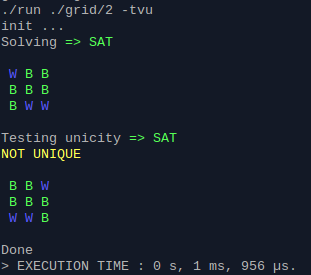
\includegraphics[scale=.6]{screen1.png}
\caption{Solution et Test d'Unicité pour la grille 2}
\end{figure}

\begin{figure}[hbtp]
\centering
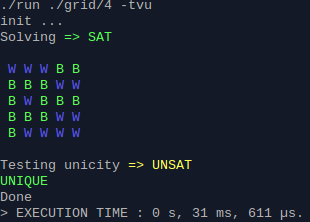
\includegraphics[scale=.6]{screen2.png}
\caption{Solution et Test d'Unicité pour la grille 4}
\end{figure}

\begin{figure}[hbtp]
\centering
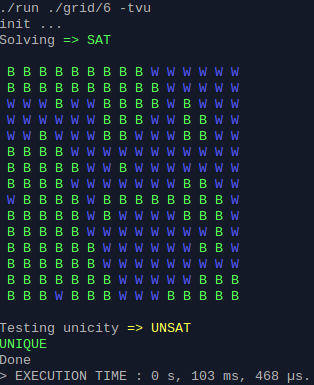
\includegraphics[scale=.6]{screen3.png}
\caption{Solution et Test d'Unicité pour la grille 6}
\end{figure}

\end{document}